% !TEX root = ../../../main.tex

\section{Dispositivi di rete}
Si sceglie, per la successiva semplicità di gestione ed una maggiore integrazione, di utilizzare dispositivi dello
stesso produttore. In particolare, si utilizzeranno dispositivi Ubiquiti UniFi.

\subsection{Centro stella}
Al centro stella, troviamo due dispositivi principali.

Il primo, il \textit{Dream Machine Pro}, è un dispositivo multiuso. Consente innanzitutto di gestire
l'intera rete, essendo una console per gli altri dispositivi in rete. Integra inoltre funzionalità di sicurezza
ed offre otto connessioni Ethernet che potrebbero essere utili per vari usi: essendo il primo dispositivo connesso
alla rete esterna, possono essere utilizzate per quelle apparecchiature che devono garantire una maggiore stabilità
nella connessione, come un server web o un sistema antifurto. In questo modo, anche se un dispositivo al di sotto
di questo fallisce, la connessione resterà attiva.

Per migliorare la stabilità della rete, utile in caso di fallimento completo della dorsale ottica, è possibile connettere
il \textit{floor distributor} del piano terreno a quattro delle porte disponibili su questo dispositivo mediante
collegamenti Ethernet Cat5e, prolungando la linea di backup.

Successivamente, connesso in cascata a questo dispositivo mediante una bretella ottica, vi è un sistema di \textit{Switch Aggregation},
ovvero uno switch di livello 2 per fibra ottica con 8 porte SFP+ da 10 Gb/s. Da questo partono le ramificazioni verso i vari \textit{floor
  distributor}.

\subsection{Floor distributor}
Ogni floor distributor sarà dotato, oltre ai dispositivi definiti nella sezione di cablaggio strutturato,
di uno \textit{Switch Pro 48}, uno switch di livello 3 dotato di 48 porte Ethernet e quattro porte SFP+.

Vista l'abbondanza di porte adatte al collegamento in fibra ottica, invece di eliminare le parti di fibra
in eccesso durante il cablaggio (si ricorda che ci sarà un cavo da 6 coppie, di cui 4 in uso, percorrente
l'intero edificio in verticale), le si potrebbero utilizzare per la creazione di un'altra linea di backup,
equivalente a quella realizzata mediante i quattro collegamenti tra armadi adiacenti. Se la rete è
configurata adeguatamente, questo aiuterebbe parecchio il traffico interno, in quanto non sarà necessario
l'attraversamento dello switch ``ottico''. Visto che molti software e sistemi operativi offrono funzionalità
di caching, una simile infrastruttura di rete aumenterebbe le performance quando vi è la necessità di installare
o aggiornare software su tutti i dispositivi aziendali, riducendo degli eventuali tempi morti.

Saranno necessari degli adattatori SFP con collegamento LC. Anche questi sono disponibili dallo stesso produttore
delle altre apparecchiature di rete.

La topologia generale è descritta dalla figura~\ref{fig:topologia}.

\newpage
\section{Resoconto}

\begin{table}[ht]
  \begin{tabular}{@{}lcrr@{}}
    \toprule
    Nome              & Tipo di dispositivo          & Quantità & Prezzo totale \\ \midrule
    Dream Machine Pro & Console/Router (L3)/Firewall & 1        & 319.00€       \\ \midrule
    Switch Pro 48     & Router (L3)                  & 5        & 2495.00€      \\ \midrule
    Switch Aggregator & Switch (L2), ottico          & 1        & 229.00€       \\ \midrule
    UF-MM-1G-20       & Adattatori SFP+              & 20       & 119.00€       \\ \bottomrule
  \end{tabular}
  \caption{Resoconto sugli apparati di rete attivi.}\label{tab:apparati-rete}
\end{table}

Come da tabella~\ref{tab:apparati-rete}, grazie alla flessibilità delle VLAN, non è necessario
l'uso di una grande quantità di dispositivi. Il subtotale per questa sezione ammonta a 3162€, IVA esclusa.
I prezzi sono stati trovati sullo store europeo di Ubiquiti. Non si includono nel conteggio eventuali
apparecchiature wireless, facilmente incorporabili.

\begin{figure}[ht]
  \centering
  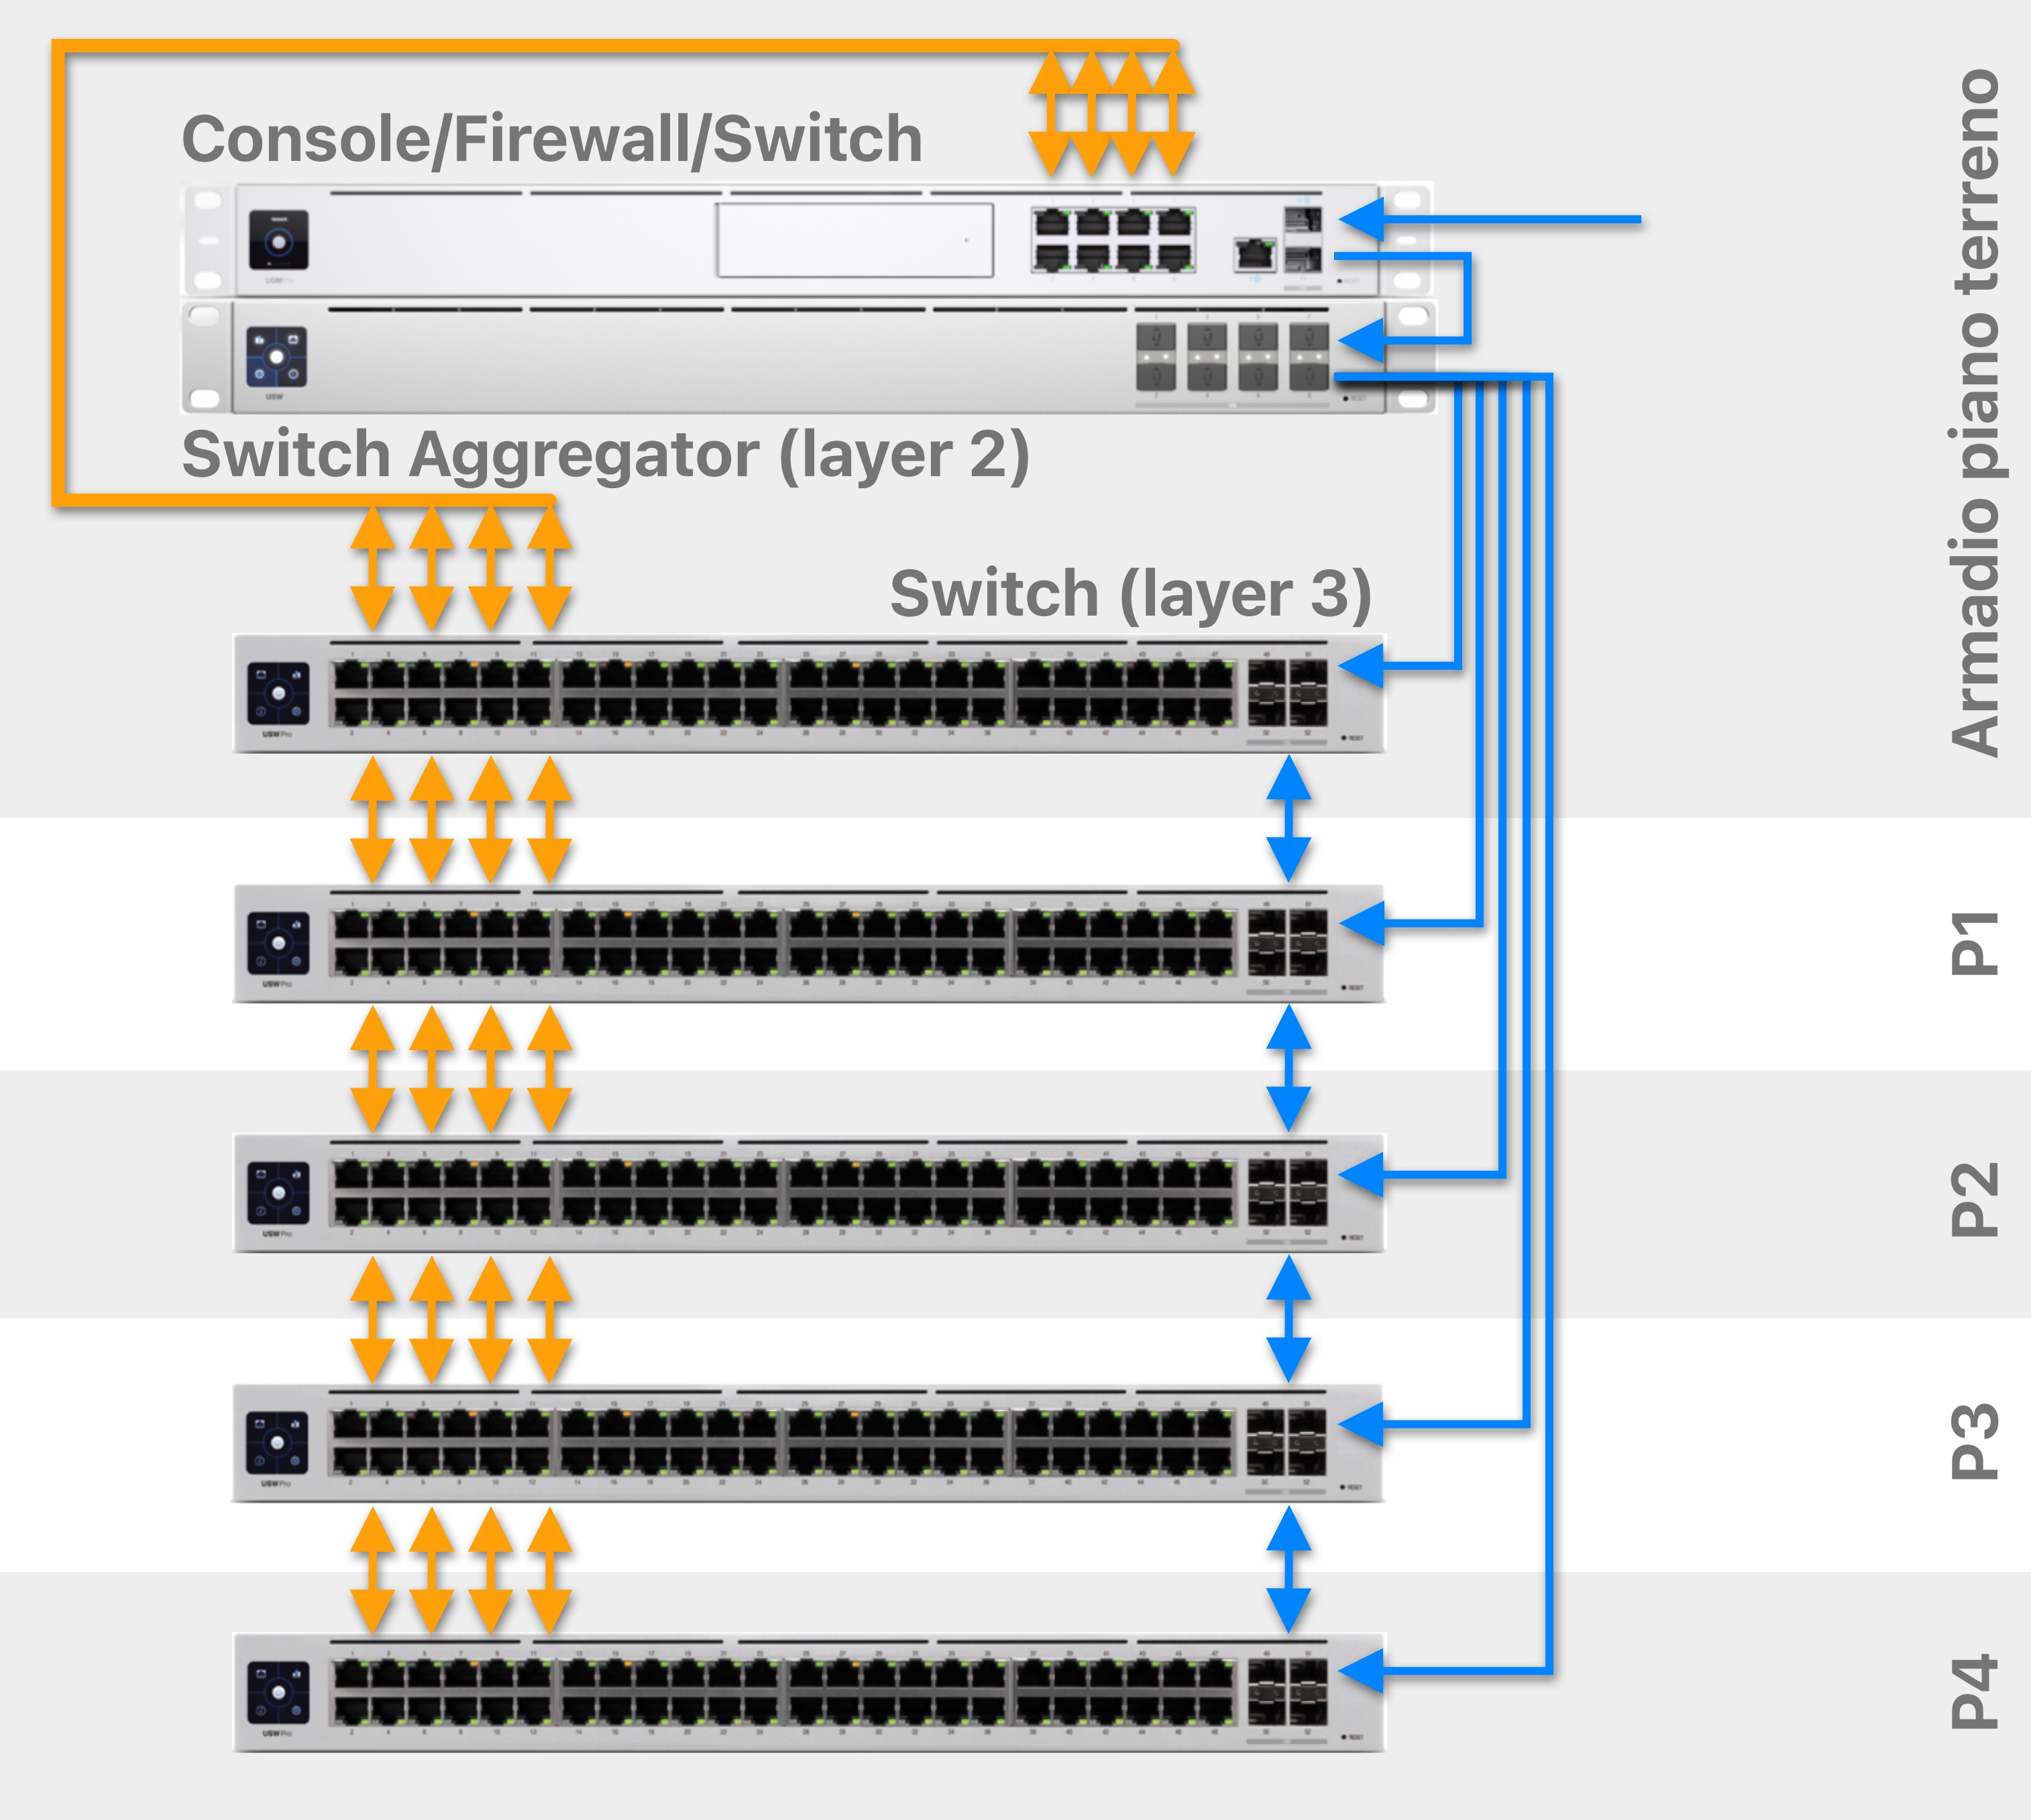
\includegraphics[height=10cm]{struttura-rete.jpg}
  \caption{
    Topologia della rete: in arancione, connessioni Ethernet su cavo Cat5e, in blu, quelle su fibra ottica multimodale. %
    Non tutte le connessioni sono obbligatorie, alcune sono ridondanti.
  }\label{fig:topologia}
\end{figure}

\newpage
\subsection{Considerazioni sulla tolleranza ai guasti}
La rottura di un router comporta la chiusura dei collegamenti di tutto il piano, ed interrompe anche
le linee di backup. Eventuali connessioni interne dovranno passare per lo switch a fibra ottica.

La rottura di uno dei due apparecchi di centro stella (o del collegamento con l'esterno) non inibisce la
comunicazione interna. Come prima specificato, è ottimale connettere le apparecchiature più importanti per l'accesso
esterno direttamente alla console (gateway), la quale ha funzionalità di switch di livello 3 su 8 prese Ethernet RJ45.

Anche se lo switch per fibra ottica dovesse smettere di funzionare, grazie all'estensione della linea di backup,
gli uffici manterranno comunque la connessone ad Internet, probabilmente con prestazioni ridotte.

Il fallimento della console principale (gateway) o della linea in fibra ottica, comporta la caduta della connessione Internet.
In generale, si ritiene difficile la totale interruzione del servizio intranet. 

Questi sistemi garantiscono inoltre, mediante l'acquisto di dispositivi aggiuntivi, una eventuale linea di backup
su rete LTE. Una simile soluzione potrebbe essere utile a mantenere attivi alcuni servizi essenziali (con ovvie limitazioni di velocità)
anche durante disservizi sulla linea fissa.
